\documentclass[a4paper, 11pt]{article}
\usepackage{amsmath}
\usepackage{graphicx}
\usepackage{geometry}
\usepackage{listings}
\geometry{scale=0.8}
\linespread{1.5}
\usepackage{hyperref}
\usepackage{listings}


\title{	
\normalfont \normalsize
\textsc{School of Data and Computer Science, Sun Yat-sen University} \\ [25pt] %textsc small capital letters
\rule{\textwidth}{0.5pt} \\[0.4cm] % Thin top horizontal rule
\huge  E07 FF Planner \\ % The assignment title
\rule{\textwidth}{2pt} \\[0.5cm] % Thick bottom horizontal rule
\author{16337102 Zilin Huang}
\date{\normalsize\today}
}

\begin{document}
\maketitle
\tableofcontents
\newpage

\section{Examples}

\subsection{Spare Tire}
\label{sec:spare-tire}

\begin{lstlisting}[title=domain\_spare\_tire.pddl,frame=single,language=lisp,numbers=left]
(define (domain spare_tire)
  (:requirements :strips :equality:typing)
  (:types physob location)
  (:predicates  (Tire ?x - physob)
		(at ?x - physob ?y - location))

(:action Remove
             :parameters (?x - physob ?y - location)
             :precondition (At ?x ?y)
             :effect (and (not (At ?x ?y)) (At ?x Ground)))

  (:action PutOn
             :parameters (?x - physob)
             :precondition (and (Tire ?x) (At ?x Ground)
                                (not (At Flat Axle)))
             :effect (and (not (At ?x Ground)) (At ?x Axle)))
  (:action LeaveOvernight
             :effect (and (not (At Spare Ground)) (not (At Spare Axle))
                          (not (At Spare Trunk)) (not (At Flat Ground))
                          (not (At Flat Axle)) (not (At Flat Trunk)) ))
 )

\end{lstlisting}
\begin{lstlisting}[title=spare\_tire.pddl,frame=single,language=lisp,numbers=left]
(define (problem prob)
 (:domain spare_tire)
 (:objects Flat Spare -physob Axle Trunk Ground - location)
 (:init (Tire Flat)(Tire Spare)(At Flat Axle)(At Spare Trunk))
 (:goal (At Spare Axle))
)


\end{lstlisting}
\begin{figure}[h]
  \centering
  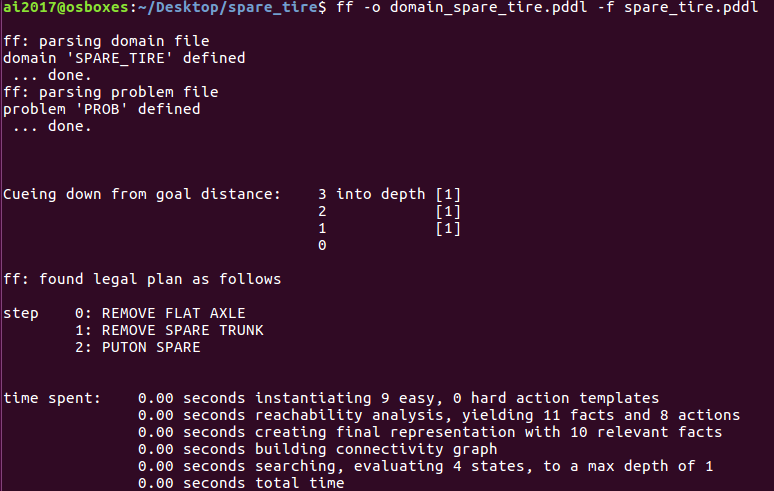
\includegraphics[width=16cm]{Pic/spare_tire}
\end{figure}

\subsection{Briefcase World}
\label{sec:briefcase-world}

Please refer to \texttt{pddl.pdf} at page 2. Please pay More attention to the usages of \texttt{forall} and \texttt{when}.

For more examples, please refer to \texttt{ff-domains.tgz} and \texttt{benchmarksV1.1.zip}. For more usages of FF planner, please refer to the documentation \texttt{pddl.pdf}.
\section{Tasks}

\subsection{8-puzzle}
\begin{figure}[ht]
  \centering
  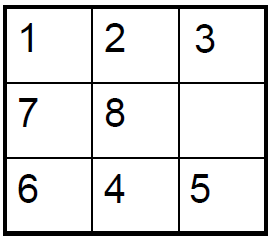
\includegraphics[width=0.4\textwidth]{Pic/puzzle}
  \qquad
  \parbox[b]{0.4\textwidth}{Please complete  \texttt{domain\_puzzle.pddl} and \texttt{puzzle.pddl} to solve the 8-puzzle problem.\\}
\end{figure}
\label{sec:8-puzzle}
\begin{lstlisting}[title=domain\_puzzle.pddl,frame=single,language=lisp,numbers=left]
(define (domain puzzle)
  (:requirements :strips :equality:typing)
  (:types num loc)
  (:predicates  ())

(:action slide
             :parameters ()
             :precondition ()
             :effect ()
 )
)
\end{lstlisting}
\begin{lstlisting}[title=domain\_puzzle.pddl,frame=single,language=lisp,numbers=left]
(define (problem prob)
 (:domain puzzle)
 (:objects )
 (:init )
 (:goal ())
)

\end{lstlisting}
\subsection{Blocks World}
\label{sec:blocksworld}
\begin{figure}[h]
  \centering
  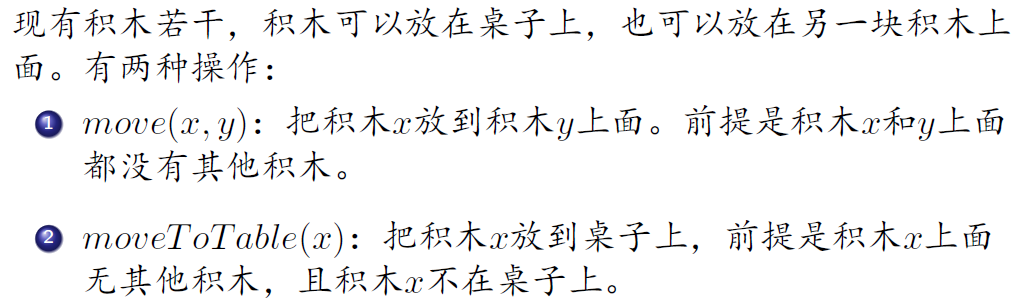
\includegraphics[width=17cm]{Pic/blocks}
\end{figure}

Please complete the file \texttt{domain\_blocks.pddl} to solve the blocks world problem. You should know the usages of \texttt{forall} and \texttt{when}.

\begin{lstlisting}[title=domain\_blocks.pddl,frame=single,language=lisp,numbers=left]
(define (domain blocks)
  (:requirements :strips :typing:equality
                 :universal-preconditions
                 :conditional-effects)
  (:types physob)
  (:predicates
  	    (ontable ?x - physob)
            (clear ?x - physob)	
	    (on ?x ?y - physob))
		
  (:action move
             :parameters (?x ?y - physob)
             :precondition ()
             :effect ()
             )

  (:action moveToTable
             :parameters (?x - physob)
             :precondition ()
             :effect ( )
 )



\end{lstlisting}

\label{sec:problem-description}

\begin{lstlisting}[title=blocks.pddl,frame=single,language=lisp,numbers=left]
(define (problem prob)
 (:domain blocks)
 (:objects A B C D E F - physob)
 (:init (clear A)(on A B)(on B C)(ontable C) (ontable D)
  (ontable F)(on E D)(clear E)(clear F)
)
 (:goal  (and (clear F) (on F A) (on A C) (ontable C)(clear E) (on E B)
         (on B D) (ontable D)) )
 )




\end{lstlisting}
Please submit a file named \textsf{E07\_YourNumber.pdf}, and send it to \textsf{ai\_2018@foxmail.com}


\section{Codes}
\begin{lstlisting}[title=domain\_puzzle.pddl,frame=single,language=lisp,numbers=left]
(define (domain puzzle)
    (:requirements :strips :equality :typing)
    (:types num loc)
    (:constants B - num)
    (:predicates (adjacent ?x - loc ?y - loc)
                 (at ?x - num ?y - loc))

(:action slide
                :parameters (?t - num ?x - loc ?y - loc)
                :precondition (and (at ?t ?x) (adjacent ?x ?y)
                                   (at B ?y))
                :effect (and (at B ?x) (at ?t ?y)
                             (not (at ?t ?x)) (not (at B ?y)) )
)
)
\end{lstlisting}

\begin{lstlisting}[title=puzzle.pddl,frame=single,language=lisp,numbers=left]
(define (problem prob)
	(:domain puzzle)
	(:objects num1 num2 num3 num4 num5 num6 num7 num8 - num
	          P1 P2 P3 P4 P5 P6 P7 P8 P9 - loc)
	(:init (at num1 P1) (at num2 P2) (at num3 P3) (at num7 P4)
	       (at num8 P5) (at B P6) (at num6 P7) (at num4 P8)
	       (at num5 P9)
	       (adjacent P1 P2) (adjacent P1 P4)
	       (adjacent P2 P1) (adjacent P2 P3)
	       (adjacent P2 P5) (adjacent P3 P2)
	       (adjacent P3 P6) (adjacent P4 P1)
	       (adjacent P4 P5) (adjacent P4 P7)
	       (adjacent P5 P2) (adjacent P5 P4)
	       (adjacent P5 P6) (adjacent P5 P8)
	       (adjacent P6 P3) (adjacent P6 P5)
	       (adjacent P6 P9) (adjacent P7 P4)
	       (adjacent P7 P8) (adjacent P8 P5)
	       (adjacent P8 P7) (adjacent P8 P9)
	       (adjacent P9 P6) (adjacent P9 P8))
	(:goal (and (at num1 P1) (at num2 P2) (at num3 P3) (at num4 P4)
	       (at num5 P5) (at num6 P6) (at num7 P7) (at num8 P8)
	       (at B P9)) )
)
\end{lstlisting}

\begin{lstlisting}[title=domain\_blocks.pddl,frame=single,language=lisp,numbers=left]
(define (domain blocks)
	(:requirements :strips :typing :equality
				   :universal-preconditions
				   :conditional-effects )
    (:types physob)
    (:predicates
                (ontable ?x - physob)
                (clear ?x - physob)
                (on ?x ?y - physob)
                )
    (:action move
                :parameters (?x ?y - physob)
                :precondition (and (clear ?y) (clear ?x))
                :effect ( and (not (clear ?y)) (on ?x ?y)
                              (forall (?z)
                                    (when (on ?x ?z)
                                    (and (not (on ?x ?z)) (clear ?z)) ))
                              (when (ontable ?x) (not (ontable ?x)) )  )
                )
    (:action moveToTable
                :parameters (?x - physob)
                :precondition (and (clear ?x) (not (ontable ?x)))
                :effect (and (ontable ?x)
                             (forall (?z)
                                    (when (on ?x ?z)
                                    (and (not (on ?x ?z)) (clear ?z)) ))
                )
)
)
\end{lstlisting}

\begin{lstlisting}[title=blocks.pddl,frame=single,language=lisp,numbers=left]
(define (problem prob)
	(:domain blocks)
	(:objects A B C D E F - physob)
	(:init (clear A) (on A B) (on B C) (ontable C) (ontable D)
	       (ontable F) (on E D) (clear E) (clear F) )
	(:goal (and (clear F) (on F A) (on A C) (ontable C)
	       (clear E) (on E B) (on B D) (ontable D) )
)
)
\end{lstlisting}

\section{Results}
\begin{figure}[h]
\centering
\includegraphics[width=15cm]{result1.png}
\caption{Pzzle}
\label{fig:1}
\end{figure}

\begin{figure}[h]
\centering
\includegraphics[width=15cm]{result2.png}
\caption{Blocks}
\label{fig:1}
\end{figure}

%\clearpage
%\bibliography{E:/Papers/LiuLab}
%\bibliographystyle{apalike}
\end{document}
%%% Local Variables:
%%% mode: latex
%%% TeX-master: t
%%% End: